\documentclass[a4paper]{report}
\usepackage{graphicx}
\usepackage[top=1cm]{geometry}
\usepackage[utf8]{vietnam}
\usepackage{hyperref}
\usepackage{bookmark}
\usepackage{booktabs}
\usepackage{tabularx}
\usepackage{adjustbox}
\usepackage{titlesec}
\usepackage{indentfirst}
\usepackage{subcaption}
\usepackage{multirow}
\usepackage[nottoc]{tocbibind}
\usepackage{fancyhdr}
\setlength{\headheight}{24.0pt}
\usepackage{tikz}
\usepackage{amsmath, amssymb, amsfonts}
\usetikzlibrary{calc} 
\usepackage{listings}
\usepackage{xcolor}
\usepackage{calc}
\usepackage{algpseudocode}
\usepackage{algorithm}
\usepackage{float}
\usepackage{cite}
\usepackage{tabularx} % thêm vào preamble

\setlength{\parindent}{0pt}
\hypersetup{
    colorlinks=true,
    linkcolor=blue,
    filecolor=magenta,      
    urlcolor=cyan,
    pdftitle={Overleaf Example},
    pdfpagemode=FullScreen,
    }
% Custom commands for math
\newcommand{\bs}{\boldsymbol}
\newcommand{\E}{\mathbb{E}}
\newcommand{\R}{\mathbb{R}}
\newcommand{\argmax}{\text{argmax}}
\newcommand{\softmax}{\text{softmax}}

% Color definitions
\definecolor{codegray}{rgb}{0.5,0.5,0.5}
\definecolor{codegreen}{rgb}{0,0.6,0}
\definecolor{codeblue}{rgb}{0,0,0.6}

% Listings configuration
\lstdefinestyle{mystyle}{
    backgroundcolor=\color{white},   
    commentstyle=\color{codegray},
    keywordstyle=\color{codeblue},
    numberstyle=\tiny\color{codegray},
    stringstyle=\color{codegreen},
    basicstyle=\ttfamily\footnotesize,
    breakatwhitespace=false,         
    breaklines=true,                 
    captionpos=b,                    
    keepspaces=true,                 
    numbers=left,                    
    numbersep=5pt,                  
    showspaces=false,                
    showstringspaces=false,
    showtabs=false,                  
    tabsize=2,
    xleftmargin=\dimexpr(\textwidth-\linewidth)/2,
    xrightmargin=\dimexpr(\textwidth-\linewidth)/2,
}

\lstnewenvironment{pseudocode}[1][]
{
    \lstset{style=mystyle,#1}
}
{}

% Chapter formatting
\titleformat{\chapter}[display]
  {\normalfont\bfseries}{}{0pt}{\Huge}
\titlespacing{\chapter}{0pt}{-50pt}{20pt}

% Page geometry
\geometry{a4paper, left=2.5cm, right=2.5cm, top=3cm, bottom=3cm}

\begin{document}
\pagestyle{empty}

% Title page
\begin{titlepage}
\begin{tikzpicture}[remember picture, overlay]
    \draw[line width=0.5pt]
    ($(current page.north west) + (1cm, -1cm)$) rectangle
    ($(current page.south east) + (-1cm, 1cm)$);
\end{tikzpicture}

\newcommand{\HRule}{\rule{\linewidth}{0.5mm}}
\centering

\textsc{\LARGE đại học quốc gia tphcm}\\[0.5cm]
\textsc{\Large trường đại học khoa học tự nhiên}\\[0.5cm]
\textsc{\Large khoa công nghệ thông tin}\\[0.8cm]

\includegraphics[scale=.40]{logo KHTN_REMAKE 1.png}\\[0.8cm] 

\begin{center}
    \Large \textbf{BÁO CÁO ĐỒ ÁN 01 - SEARCH ALGORITHMS}\\[0.5em]
    % \Large \textbf{IMPROVING LANGUAGE UNDERSTANDING BY}\\[0.3em]
    % \Large \textbf{GENERATIVE PRE-TRAINING}\\[0.3em]
    % \large \textbf{Nghiên cứu và Phân tích Khung làm việc GPT-1}
\end{center}
\hrule
\vspace{1em}

\vspace{1cm}

\textbf{\large Môn học: CSC14003 – Cơ sở Trí tuệ Nhân tạo}\\[0.5cm]

\begin{minipage}[t]{0.4\textwidth}
\begin{flushleft} \large
\emph{Sinh viên:}\\
\emph{Hoàng Minh Trung - 23122014}\\
\emph{Nguyễn Gia Bảo - 23122015}\\
\emph{Bùi Duy Bảo - 23122021}\\
\emph{Huỳnh Trung Kiệt - 23122039}\\
\end{flushleft}
\end{minipage}
~
\begin{minipage}[t]{0.4\textwidth}
\begin{flushright} \large
\emph{GVHD:} \\
\emph{GS. Lê Hoài Bắc}\\
\emph{ThS. Lê Nhựt Nam}
\end{flushright}
\end{minipage}\\[2cm]

{\large \today}\\[1cm]
\vfill
\end{titlepage}


% Chèn sau \end{titlepage}

\pagestyle{plain} % Bật số trang cho mục lục

%---------------- Mục lục ----------------%
\tableofcontents
\thispagestyle{plain} % Số trang xuất hiện ở trang mục lục

%---------------- Danh sách hình ảnh & bảng ----------------%
\listoffigures
\listoftables

\newpage
\setcounter{page}{1} % Bắt đầu số trang từ 1 sau mục lục
\pagestyle{fancy} % Bật fancy header/footer nếu muốn
\fancyhf{}
\fancyhead[L]{Báo cáo đồ án}
\fancyhead[R]{\thepage}
\renewcommand{\headrulewidth}{0.4pt}
\renewcommand{\footrulewidth}{0pt}


%---------------- 1. PROJECT OVERVIEW ----------------%
\chapter{Giới thiệu đồ án}
\section{Tổng quan đề tài}
Trình bày tóm tắt về mục tiêu của đồ án, lý do chọn chủ đề, ý nghĩa của việc nghiên cứu các thuật toán tìm kiếm bầy đàn (Swarm Intelligence).

\section{Mục tiêu học tập}
\begin{itemize}
    \item Hiểu cơ sở lý thuyết của các thuật toán trí tuệ bầy đàn.
    \item Cài đặt các thuật toán tối ưu hoá theo tự nhiên bằng NumPy.
    \item So sánh hiệu năng giữa các thuật toán swarm và các thuật toán tìm kiếm truyền thống.
\end{itemize}

%---------------- 2. PHÂN CÔNG CÔNG VIỆC ----------------%
\chapter{Phân công công việc}
\section{Bảng phân công}


\section{Tự đánh giá}
Trình bày mức độ hoàn thành, tinh thần làm việc nhóm, và các khó khăn gặp phải.

%---------------- 3. MÔ TẢ THUẬT TOÁN ----------------%
\chapter{Mô tả chi tiết các thuật toán}
\section{Ant Colony Optimization (ACO)}
Trình bày công thức, nguyên lý pheromone update, heuristic.


\section{Particle Swarm Optimization (PSO)}
Trình bày công thức cập nhật vận tốc, vị trí, giải thích các tham số.

\section{Thuật toán Artificial Bee Colony (ABC)}

\subsection{Nguyên lý cơ bản}
Thuật toán \textit{Artificial Bee Colony} (ABC) được đề xuất bởi Derviş Karaboğa vào năm 2005, là một thuật toán tối ưu hóa dựa trên hành vi tìm kiếm thức ăn (foraging behavior) của đàn ong mật. Trong tự nhiên, đàn ong có khả năng tìm kiếm và khai thác nguồn mật một cách tối ưu thông qua cơ chế cộng tác xã hội, truyền tin bằng "vũ điệu lắc lư" (waggle dance) và khả năng thích nghi cao với môi trường. Mô hình ABC mô phỏng hành vi này để giải quyết các bài toán tối ưu hoá phi tuyến, phi đạo hàm, hoặc đa cực trị.

Trong mô hình ABC, quần thể ong nhân tạo được chia thành ba nhóm:
\begin{itemize}
    \item \textbf{Ong thu việc (Employed Bees):} Mỗi ong tương ứng với một nguồn thức ăn (một lời giải ứng viên). Chúng ghi nhớ vị trí nguồn của mình, di chuyển đến đó để thu thập thông tin và đánh giá “lượng mật” (giá trị hàm mục tiêu). Sau đó, ong quay lại tổ và thực hiện “vũ điệu” để chia sẻ thông tin với các ong khác.
    \item \textbf{Ong quan sát (Onlooker Bees):} Nhóm ong này ở trong tổ, quan sát các điệu nhảy của ong thu việc để quyết định nguồn thức ăn nào đáng đến hơn. Xác suất chọn của mỗi ong quan sát tỉ lệ thuận với chất lượng (fitness) của nguồn thức ăn được quảng bá.
    \item \textbf{Ong do thám (Scout Bees):} Khi một nguồn thức ăn không còn được cải thiện sau một số vòng lặp nhất định (\textit{limit}), ong thu việc tương ứng sẽ trở thành ong do thám, bỏ nguồn cũ và tìm kiếm ngẫu nhiên một nguồn thức ăn mới trong không gian nghiệm.
\end{itemize}

\subsection{Mô hình và các bước chính của thuật toán}
Giả sử bài toán tối ưu có hàm mục tiêu $f: \mathbb{R}^n \rightarrow \mathbb{R}$, cần tìm nghiệm tối ưu (tối đa hoặc tối thiểu). Trong ABC, một nghiệm (hay nguồn thức ăn) được biểu diễn bởi vector:
\[
X_i = (x_{i,1}, x_{i,2}, \ldots, x_{i,n}), \quad i = 1, 2, \ldots, SN,
\]
trong đó $SN$ là kích thước quần thể (số lượng nguồn thức ăn, cũng là số lượng ong thu việc).

Quá trình hoạt động của ABC bao gồm các bước chính như sau:

\begin{enumerate}
    \item \textbf{Khởi tạo quần thể ban đầu:}  
    Sinh ngẫu nhiên $SN$ nguồn thức ăn trong phạm vi tìm kiếm $[lb, ub]$, với công thức:
    \[
    x_{i,k} = lb_k + \mathrm{rand}(0,1)\times(ub_k - lb_k),
    \]
    trong đó $lb_k$ và $ub_k$ là giới hạn dưới và trên của chiều thứ $k$.

    \item \textbf{Pha Ong Thu Việc (Employed Bee Phase):}  
    Mỗi ong thu việc $i$ tạo một nghiệm ứng viên mới $V_i$ dựa trên nghiệm hiện tại $X_i$ và một nghiệm ngẫu nhiên khác $X_j$ ($i \neq j$):
    \[
    v_{i,k} = x_{i,k} + \Phi_{i,k}(x_{i,k} - x_{j,k}),
    \]
    trong đó $\Phi_{i,k}$ là một số ngẫu nhiên trong đoạn $[-1,1]$.  
    Sau đó, áp dụng lựa chọn tham lam (greedy selection):  
    Nếu $f(V_i)$ tốt hơn $f(X_i)$ thì thay $X_i \leftarrow V_i$, ngược lại giữ nguyên.

    \item \textbf{Pha Ong Quan Sát (Onlooker Bee Phase):}  
    Mỗi ong quan sát chọn một nguồn thức ăn $X_i$ để khám phá, dựa trên xác suất tỉ lệ với độ phù hợp (fitness) của nó:
    \[
    P_i = \frac{\mathrm{fit}_i}{\sum_{j=1}^{SN} \mathrm{fit}_j}.
    \]
    Cơ chế chọn này được gọi là \textit{roulette wheel selection}. Sau khi chọn, ong quan sát cũng tạo một nghiệm mới $V_i$ tương tự công thức ở trên, đánh giá và cập nhật theo chiến lược tham lam như trong pha ong thu việc.

    \item \textbf{Pha Ong Do Thám (Scout Bee Phase):}  
    Nếu một nguồn thức ăn $X_i$ không được cải thiện sau một số vòng lặp nhất định (theo biến đếm $trial_i$), nó được xem là bị “bỏ hoang”. Khi đó, ong thu việc tương ứng trở thành ong do thám và tìm kiếm một nguồn mới:
    \[
    x_{i,k} = lb_k + \mathrm{rand}(0,1)\times(ub_k - lb_k).
    \]

    \item \textbf{Cập nhật nghiệm tốt nhất:}  
    Sau mỗi chu kỳ (một vòng gồm ba pha trên), thuật toán lưu lại nghiệm có giá trị tốt nhất (nguồn có lượng mật cao nhất) được tìm thấy cho đến thời điểm hiện tại.
\end{enumerate}

Quy trình này được lặp lại cho đến khi thoả mãn điều kiện dừng (ví dụ: đạt số vòng lặp cực đại $maxIter$, hoặc sai số hội tụ nhỏ hơn ngưỡng đặt trước).

\subsection{Giải thích chi tiết và cơ chế hoạt động}
Thuật toán ABC là một thuật toán dựa trên quần thể (population-based algorithm). Mỗi cá thể trong quần thể đại diện cho một nghiệm ứng viên của bài toán tối ưu. Quá trình tiến hoá của quần thể diễn ra thông qua ba pha tương ứng với hành vi của ba loại ong:

\begin{itemize}
    \item \textbf{Pha tìm kiếm cục bộ (Employed + Onlooker):}  
    Hai pha đầu cho phép quần thể khai thác vùng nghiệm xung quanh các nguồn tốt hiện có. Mỗi lần cập nhật $V_i$ giúp thuật toán dịch chuyển nghiệm sang vùng lân cận tiềm năng hơn.
    
    \item \textbf{Pha khám phá toàn cục (Scout):}  
    Giúp thuật toán tránh bị kẹt trong cực trị địa phương bằng cách thay thế các nghiệm không tiến triển bằng nghiệm ngẫu nhiên mới, mở rộng phạm vi tìm kiếm trong không gian giải pháp.

    \item \textbf{Chiến lược chọn lọc:}  
    ABC áp dụng quy tắc tham lam nhằm duy trì hoặc cải thiện chất lượng trung bình quần thể qua mỗi chu kỳ, đồng thời đảm bảo tính ổn định của tiến trình tối ưu.
\end{itemize}

\subsection{Mô hình toán học tổng quát}
Công thức cập nhật nghiệm của ABC có thể tổng quát hóa như sau:
\[
V_i = X_i + \Phi_i \odot (X_i - X_j),
\]
trong đó $\Phi_i$ là vector ngẫu nhiên có các phần tử trong $[-1,1]$, và $\odot$ biểu thị phép nhân từng phần tử.  
Fitness của một nghiệm $X_i$ trong bài toán \textit{minimization} được xác định bằng:
\[
\mathrm{fit}_i = 
\begin{cases}
\dfrac{1}{1 + f(X_i)}, & \text{nếu } f(X_i) \ge 0,\\[1em]
1 + |f(X_i)|, & \text{nếu } f(X_i) < 0.
\end{cases}
\]
Nhờ đó, bài toán tối thiểu hóa có thể được chuyển đổi về dạng “cực đại hóa độ phù hợp”.

\subsection{Tóm tắt thuật toán}
\begin{center}
\begin{tabular}{p{0.95\linewidth}}
\textbf{Bước 1:} Khởi tạo $SN$ nguồn thức ăn ngẫu nhiên trong không gian tìm kiếm. \\[0.4em]
\textbf{Bước 2:} Với mỗi nguồn, xác định giá trị hàm mục tiêu và fitness. \\[0.4em]
\textbf{Bước 3:} \textit{Pha Ong Thu Việc:} Sinh nghiệm mới, so sánh và cập nhật. \\[0.4em]
\textbf{Bước 4:} \textit{Pha Ong Quan Sát:} Lựa chọn nguồn theo xác suất $P_i$, sinh nghiệm mới và cập nhật. \\[0.4em]
\textbf{Bước 5:} \textit{Pha Ong Do Thám:} Với các nguồn không cải thiện sau “limit” vòng, sinh nguồn mới ngẫu nhiên. \\[0.4em]
\textbf{Bước 6:} Cập nhật nghiệm tốt nhất toàn cục. \\[0.4em]
\textbf{Bước 7:} Lặp lại từ Bước 3 cho đến khi đạt điều kiện dừng. \\
\end{tabular}
\end{center}

\subsection{Đặc điểm nổi bật}
\begin{itemize}
    \item Thuật toán đơn giản, dễ hiểu và dễ cài đặt.
    \item Có khả năng cân bằng giữa \textbf{khai thác cục bộ} và \textbf{khám phá toàn cục}.
    \item Ít tham số điều chỉnh (chủ yếu gồm $SN$, $limit$, và $maxIter$).
    \item Ứng dụng hiệu quả trong các bài toán tối ưu liên tục, rời rạc, hoặc tối ưu tổ hợp.
\end{itemize}

\subsection{Tổng kết}
Như vậy, thuật toán ABC mô phỏng chân thực quá trình tự nhiên của đàn ong trong việc tối ưu hóa hành vi kiếm ăn. Mỗi vòng lặp là một chu kỳ “tìm kiếm – chọn lọc – khám phá” giúp quần thể dần hội tụ đến nghiệm tối ưu. Nhờ đặc tính đơn giản nhưng mạnh mẽ, ABC đã được ứng dụng trong nhiều lĩnh vực như tối ưu hoá hàm số, chọn đặc trưng, lập lịch, và huấn luyện mô hình học máy.


\section{Firefly Algorithm (FA)}

\section{Cuckoo Search (CS)}

%---------------- 4. THUẬT TOÁN TRUYỀN THỐNG ----------------%
\chapter{Thuật toán tìm kiếm truyền thống để so sánh}
\section{Hill Climbing}
\section{Simulated Annealing}
\section{Thuật toán Di truyền (Genetic Algorithm - GA)}

\subsection{Nguyên lý cơ bản}
Thuật toán \textit{Di truyền} (\textit{Genetic Algorithm} - GA) là một phương pháp tối ưu hóa ngẫu nhiên được đề xuất bởi John Holland vào những năm 1970, dựa trên quá trình \textbf{chọn lọc tự nhiên} và \textbf{tiến hoá sinh học}.  
GA thuộc nhóm các thuật toán tiến hoá (\textit{Evolutionary Algorithms} - EA), mô phỏng quá trình thích nghi của sinh vật trong tự nhiên để dần dần tìm ra nghiệm tối ưu cho một bài toán.

Trong GA, mỗi nghiệm (hay cá thể) được xem như một \textbf{nhiễm sắc thể} (chromosome), chứa tập hợp các \textbf{gen} đại diện cho các tham số của bài toán. Tập hợp tất cả các cá thể tạo thành \textbf{quần thể} (population).  
Quá trình tiến hoá của quần thể diễn ra thông qua các phép toán di truyền chính:
\begin{itemize}
    \item \textbf{Chọn lọc (Selection):} Lựa chọn các cá thể có độ thích nghi cao hơn để sinh sản.
    \item \textbf{Lai ghép (Crossover):} Kết hợp thông tin di truyền giữa hai cá thể cha mẹ để tạo ra cá thể con mới.
    \item \textbf{Đột biến (Mutation):} Thay đổi ngẫu nhiên một phần nhỏ của nhiễm sắc thể nhằm duy trì đa dạng di truyền.
\end{itemize}

Quá trình trên được lặp lại qua nhiều thế hệ (generations), giúp quần thể dần hội tụ đến nghiệm tối ưu.

\subsection{Mô hình và các bước chính của thuật toán}
Giả sử cần tối ưu hàm mục tiêu $f: \mathbb{R}^n \rightarrow \mathbb{R}$. Mỗi cá thể trong quần thể được biểu diễn bằng một vector:
\[
X_i = (x_{i,1}, x_{i,2}, \ldots, x_{i,n}), \quad i = 1, 2, \ldots, N,
\]
trong đó $N$ là kích thước quần thể.  

Thuật toán GA hoạt động theo các bước chính như sau:

\begin{enumerate}
    \item \textbf{Khởi tạo quần thể ban đầu:}  
    Sinh ngẫu nhiên $N$ cá thể trong không gian tìm kiếm $[lb, ub]$ theo công thức:
    \[
    x_{i,k} = lb_k + \mathrm{rand}(0,1)\times(ub_k - lb_k).
    \]
    Mỗi cá thể được đánh giá bằng \textbf{hàm thích nghi} (fitness function) dựa trên giá trị $f(X_i)$.

    \item \textbf{Chọn lọc (Selection):}  
    Lựa chọn cá thể tốt hơn để sinh sản, thường dựa theo xác suất tỉ lệ thuận với giá trị fitness:
    \[
    P_i = \frac{\mathrm{fit}_i}{\sum_{j=1}^{N}\mathrm{fit}_j}.
    \]
    Các phương pháp chọn lọc phổ biến gồm: \textit{roulette wheel selection}, \textit{tournament selection}, hoặc \textit{rank selection}.

    \item \textbf{Lai ghép (Crossover):}  
    Chọn ngẫu nhiên hai cá thể cha mẹ $(X_p, X_q)$ và trao đổi gen của chúng để tạo cá thể con mới.  
    Với xác suất lai ghép $p_c$, phép lai có thể được thực hiện theo nhiều kiểu:
    \begin{itemize}
        \item \textit{One-point crossover:} Chọn ngẫu nhiên một vị trí chia, phần trước lấy từ cha, phần sau lấy từ mẹ.
        \item \textit{Two-point crossover:} Chọn hai vị trí chia, hoán đổi đoạn giữa cho nhau.
        \item \textit{Uniform crossover:} Mỗi gen được chọn ngẫu nhiên từ một trong hai cha mẹ.
    \end{itemize}

    \item \textbf{Đột biến (Mutation):}  
    Với xác suất $p_m$ nhỏ, thay đổi ngẫu nhiên một hoặc vài gen trong nhiễm sắc thể con:
    \[
    x'_{i,k} = 
    \begin{cases}
        lb_k + \mathrm{rand}(0,1)\times(ub_k - lb_k), & \text{với xác suất } p_m,\\
        x_{i,k}, & \text{ngược lại.}
    \end{cases}
    \]
    Đột biến giúp duy trì tính đa dạng trong quần thể và tránh bị kẹt ở cực trị địa phương.

    \item \textbf{Cập nhật thế hệ mới:}  
    Tạo quần thể mới từ các cá thể con, có thể kết hợp với một số cá thể tốt nhất từ thế hệ trước (kỹ thuật \textit{elitism}) để đảm bảo nghiệm tốt không bị mất.

    \item \textbf{Điều kiện dừng:}  
    Thuật toán dừng khi đạt số thế hệ tối đa ($maxGen$), hoặc khi giá trị fitness không còn cải thiện đáng kể.
\end{enumerate}

\subsection{Giải thích cơ chế hoạt động}
Thuật toán GA mô phỏng tiến hoá tự nhiên: các cá thể mạnh (nghiệm tốt) có khả năng sinh sản cao hơn, truyền gen tốt sang thế hệ sau.  
Sự kết hợp giữa \textit{chọn lọc} và \textit{lai ghép} giúp quần thể khai thác vùng nghiệm tiềm năng, trong khi \textit{đột biến} đảm bảo khả năng khám phá toàn cục.  
Nhờ vậy, GA đạt được sự cân bằng giữa hai yếu tố:
\begin{itemize}
    \item \textbf{Khai thác cục bộ (exploitation):} Cải thiện nghiệm hiện có.
    \item \textbf{Khám phá toàn cục (exploration):} Tìm kiếm nghiệm mới trong không gian lớn.
\end{itemize}

\subsection{Mô hình toán học tổng quát}
Quá trình tạo cá thể mới trong GA có thể được mô tả như sau:
\[
X^{(t+1)} = \mathrm{Mutation}(\mathrm{Crossover}(\mathrm{Selection}(X^{(t)}))).
\]
Trong đó $t$ là số thế hệ.  
Fitness được định nghĩa tùy thuộc vào bài toán (minimization hoặc maximization).  
Đối với bài toán tối thiểu hoá, ta có thể quy đổi về dạng độ phù hợp như sau:
\[
\mathrm{fit}_i = \frac{1}{1 + f(X_i)}.
\]

\subsection{Tóm tắt thuật toán}
\begin{center}
\begin{tabular}{p{0.95\linewidth}}
\textbf{Bước 1:} Khởi tạo quần thể ban đầu ngẫu nhiên. \\[0.4em]
\textbf{Bước 2:} Đánh giá fitness của từng cá thể. \\[0.4em]
\textbf{Bước 3:} Chọn lọc cá thể cha mẹ dựa trên fitness. \\[0.4em]
\textbf{Bước 4:} Thực hiện lai ghép để sinh cá thể con mới. \\[0.4em]
\textbf{Bước 5:} Thực hiện đột biến ngẫu nhiên với xác suất $p_m$. \\[0.4em]
\textbf{Bước 6:} Tạo thế hệ mới (có thể áp dụng elitism). \\[0.4em]
\textbf{Bước 7:} Kiểm tra điều kiện dừng, nếu chưa thoả mãn thì quay lại Bước 2. \\
\end{tabular}
\end{center}

\subsection{Đặc điểm nổi bật}
\begin{itemize}
    \item Phù hợp với các bài toán tối ưu phức tạp, phi tuyến, không khả vi.
    \item Dễ mở rộng và kết hợp với các thuật toán khác như \textit{hill climbing}, \textit{simulated annealing}, hoặc \textit{neural networks}.
    \item Có khả năng tìm nghiệm gần tối ưu trong không gian lớn, đặc biệt khi hàm mục tiêu có nhiều cực trị địa phương.
    \item Các tham số chính cần điều chỉnh gồm: kích thước quần thể $N$, xác suất lai $p_c$, xác suất đột biến $p_m$, và số thế hệ $maxGen$.
\end{itemize}

\subsection{Tổng kết}
Thuật toán di truyền là một công cụ tối ưu hóa mạnh mẽ dựa trên nguyên lý tiến hóa tự nhiên.  
Nhờ sự kết hợp linh hoạt giữa chọn lọc, lai ghép và đột biến, GA có khả năng tự thích nghi và khám phá không gian nghiệm hiệu quả.  
Tuy không đảm bảo luôn tìm được nghiệm tối ưu toàn cục, nhưng GA thường mang lại nghiệm tốt trong thời gian hợp lý - đặc biệt phù hợp với các bài toán phức tạp, đa cực trị hoặc có không gian nghiệm rời rạc.

\section{Breadth-first Search}
\section{A Star (A*)} 

%---------------- 5. THỬ NGHIỆM & KẾT QUẢ ----------------%
\chapter{Thử nghiệm và kết quả}
\section{Bài toán thử nghiệm}
\begin{itemize}
    \item \textbf{Continuous:} Sphere, Rastrigin, Rosenbrock, Ackley.
    \item \textbf{Discrete:} TSP, Knapsack, Graph Coloring.
\end{itemize}

\section{Phương pháp thực nghiệm}
Trình bày cấu hình máy, tham số, số lần chạy trung bình.

\section{Kết quả}
Đưa vào các bảng và biểu đồ (Matplotlib/Seaborn).
\begin{figure}[H]
\centering
\includegraphics[width=0.8\textwidth]{pso_convergence.png}
\caption{Đồ thị hội tụ của PSO}
\end{figure}

\subsection{So sánh ABC vs GA trên hàm Rastrigin}
Hàm \textbf{Rastrigin} là hàm chuẩn để đánh giá khả năng tránh kẹt cực trị địa phương do có nhiều điểm cực trị. Bảng dưới đây tổng hợp kết quả (tối thiểu hoá) của \textit{Artificial Bee Colony (ABC)} và \textit{Genetic Algorithm (GA)} trên Rastrigin với miền $[-5.12, 5.12]^d$.

\begin{table}[H]
\centering
\caption{So sánh hiệu năng ABC vs GA trên Rastrigin (kết quả thực nghiệm).}
\begin{adjustbox}{max width=\textwidth}
\begin{tabular}{lcccc}
    oprule
Thuật toán & Best & Mean & Std & Thời gian (s) \\
\midrule
ABC & 1.363023 & 2.920624 & 1.268702 & 0.4639 \\
GA  & 24.618936 & 47.009612 & 14.204366 & 0.2981 \\
\bottomrule
\end{tabular}
\end{adjustbox}
\vspace{0.3em}
\footnotesize{Ghi chú: \textit{Best} = giá trị nhỏ nhất; \textit{Mean/Std} trên 5 lần chạy; thời gian là trung bình (\texttt{python main.py abc\_vs\_ga}, dim=10, max\_iter=100).}
\end{table}

\paragraph{Nhận xét nhanh:}
\begin{itemize}
    \item \textbf{ABC} đạt kết quả tốt và ổn định hơn (Std nhỏ) nhờ cơ chế do thám giúp thoát cực trị địa phương.
    \item \textbf{GA} cần nhiều thế hệ để khuếch tán gen tốt; biến thiên lớn nếu tham số lai/đột biến chưa tối ưu.
    \item ABC cần ít vòng lặp hơn để đạt ngưỡng hội tụ trong cấu hình này.
    \item GA có thể cải thiện với elitism mạnh, BLX-\alpha/SBX cho không gian liên tục.
\end{itemize}

\begin{figure}[H]
    \centering
    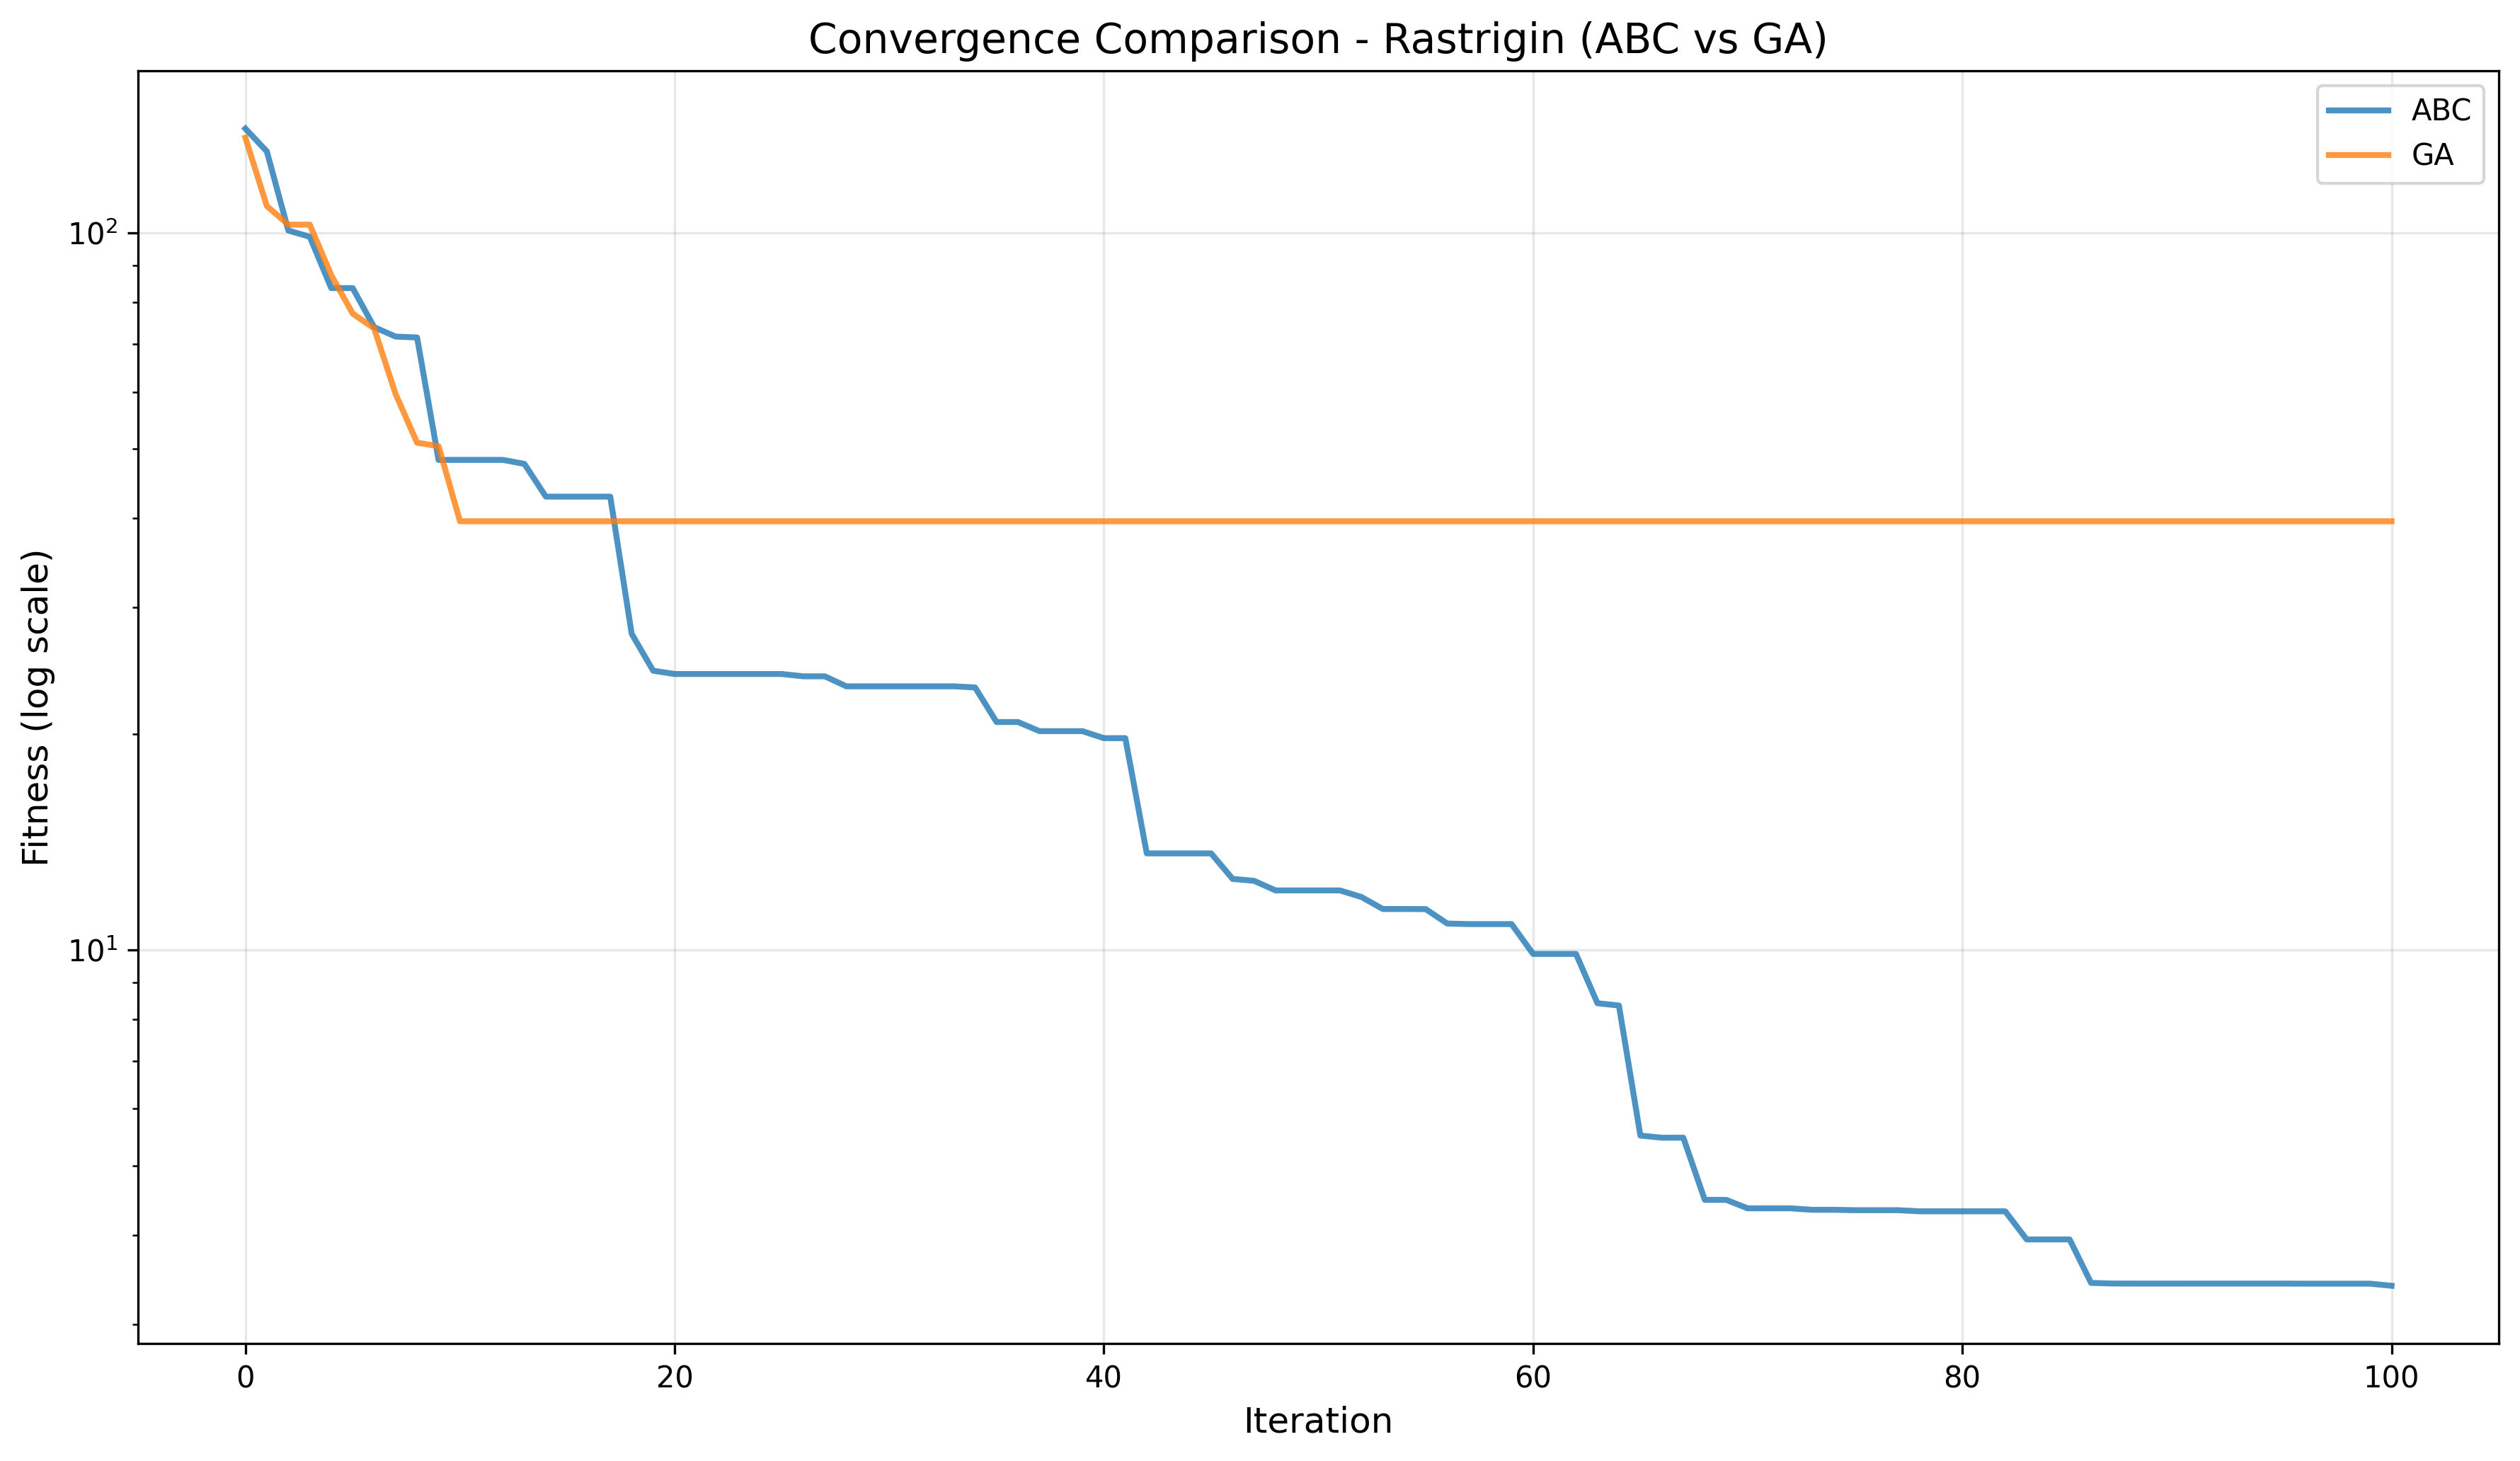
\includegraphics[width=0.85\textwidth]{figures/rastrigin_(abc_vs_ga)_convergence.png}
    \caption{Đường hội tụ (log-scale) ABC vs GA trên Rastrigin (10D).}
\end{figure}

\begin{figure}[H]
    \centering
    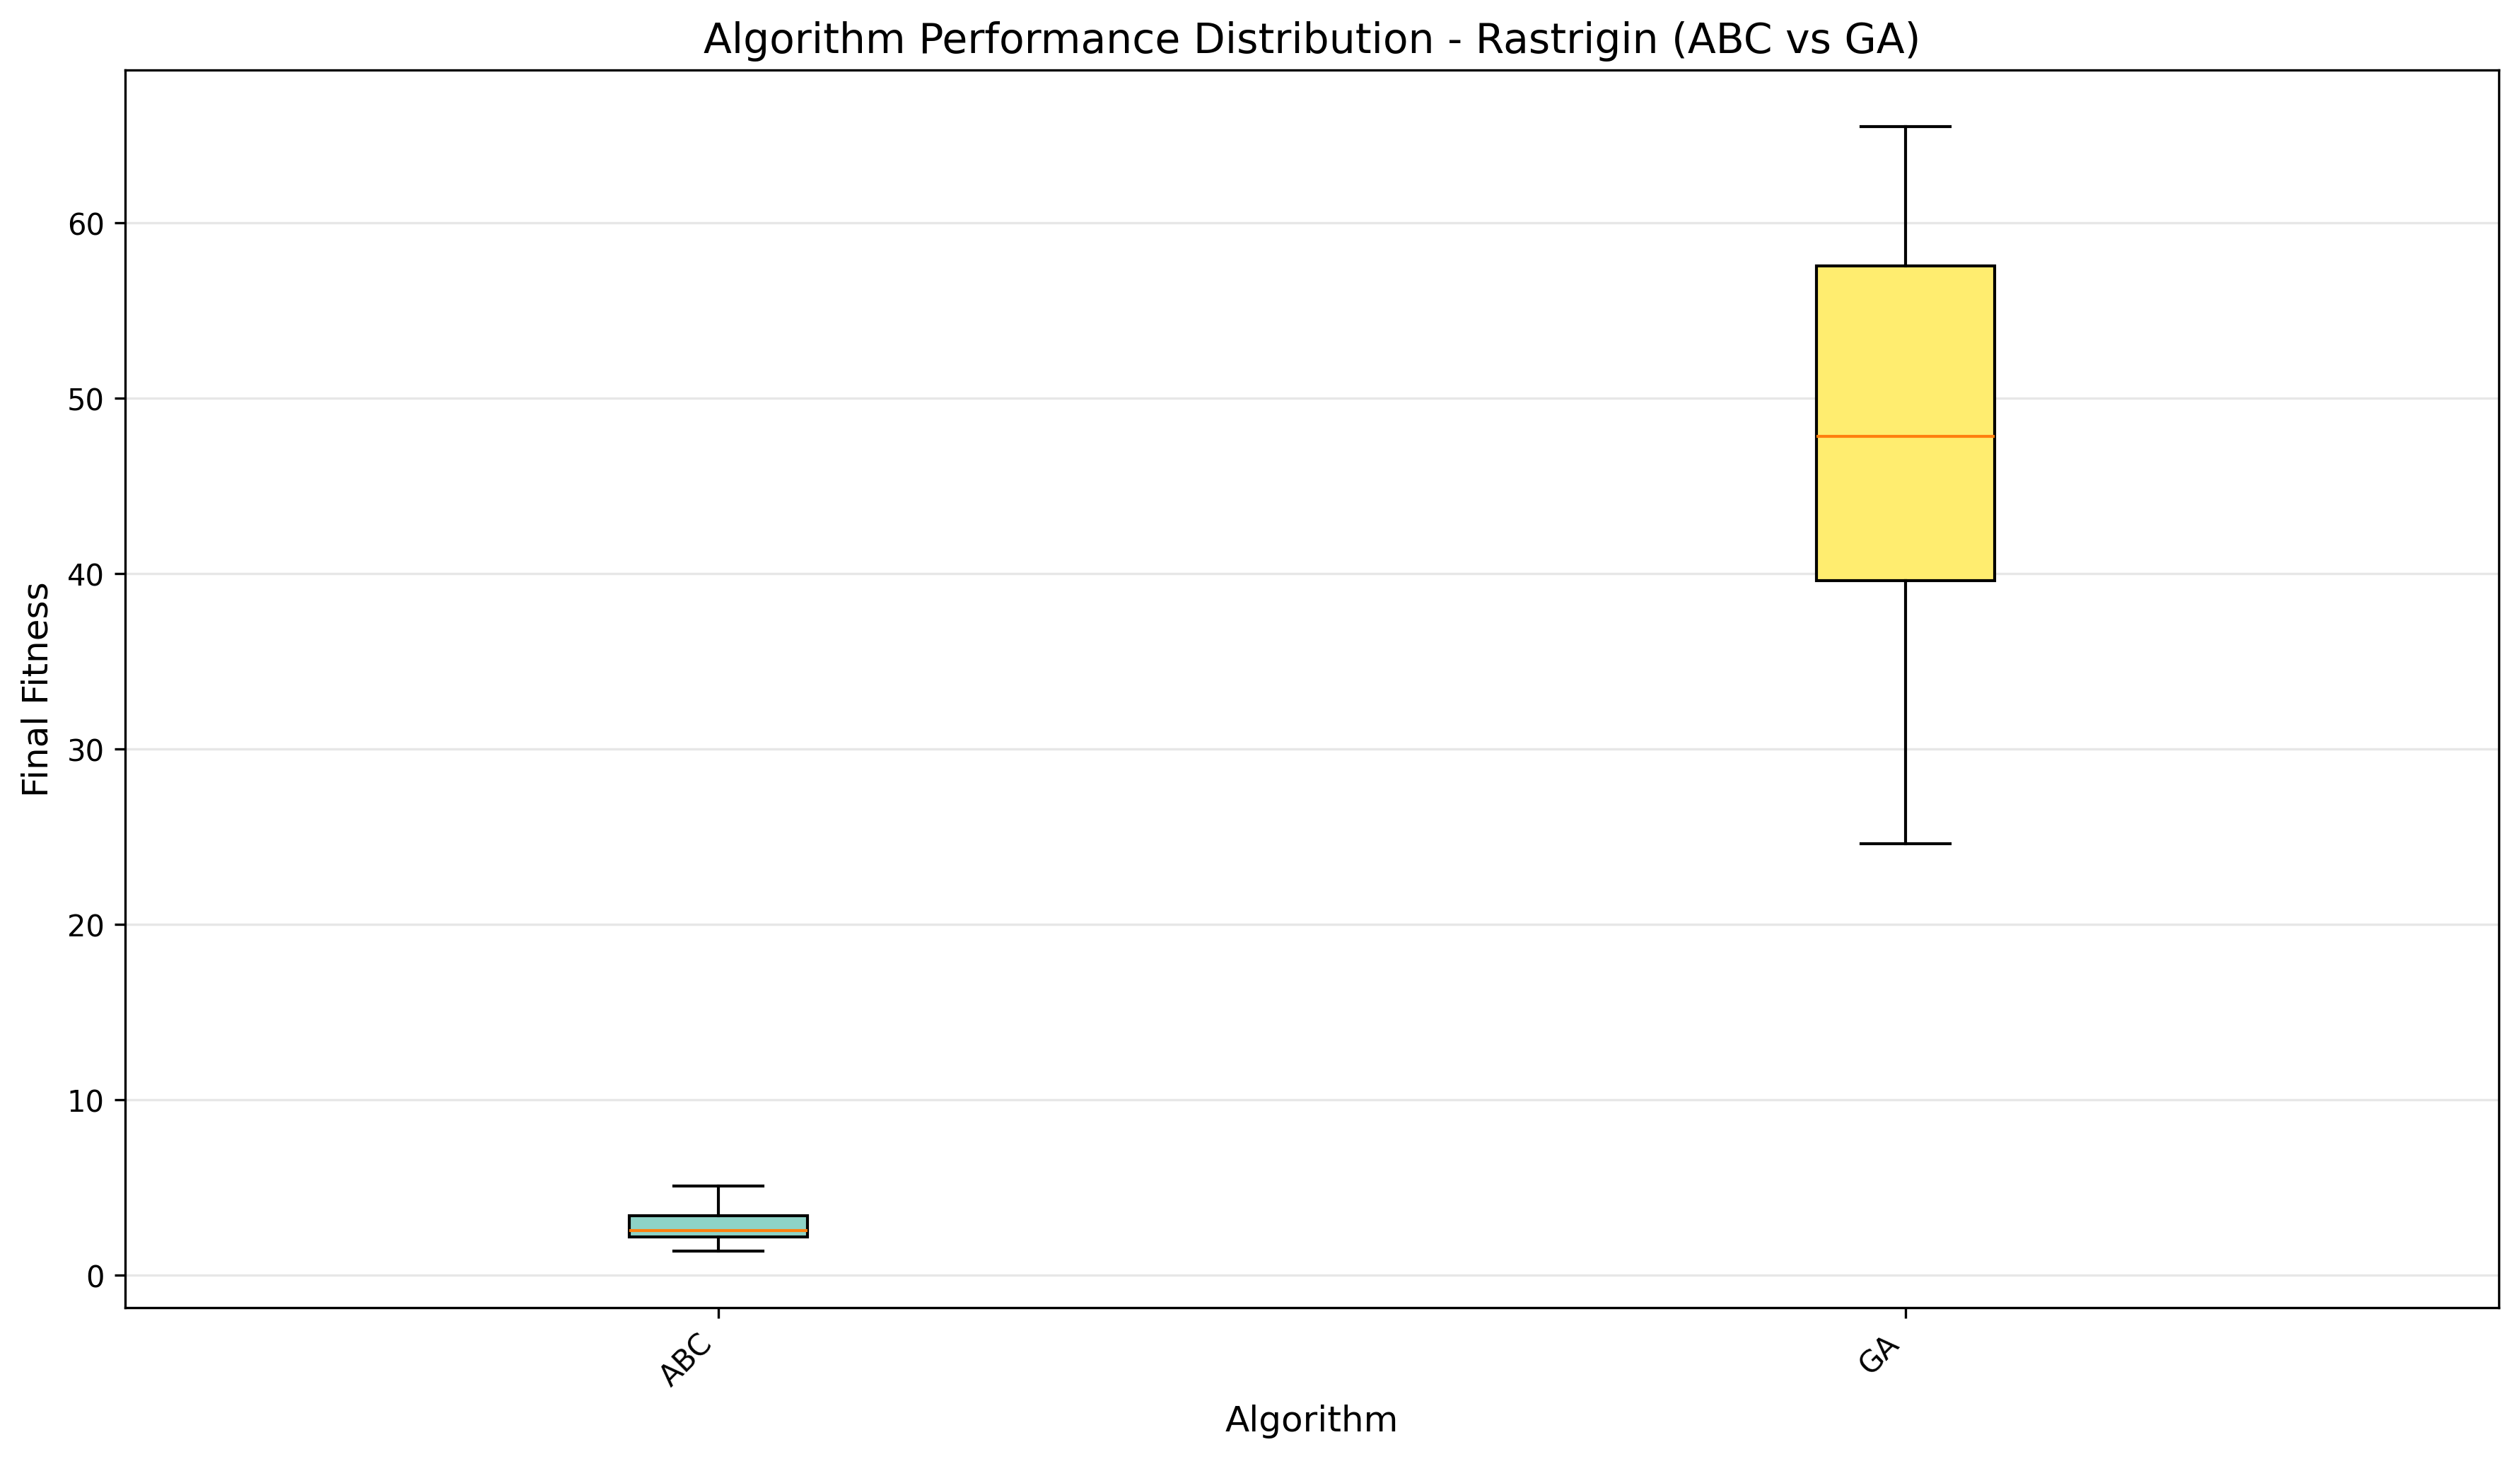
\includegraphics[width=0.75\textwidth]{figures/rastrigin_(abc_vs_ga)_boxplot.png}
    \caption{Phân bố giá trị cuối sau hội tụ (Boxplot) trên Rastrigin (10D).}
\end{figure}

\paragraph{Phân tích sâu hơn:} ABC cập nhật theo chênh lệch $(X_i - X_j)$ tạo bước nhảy thích nghi; GA phụ thuộc vào lai/đột biến nên dễ sinh nhiều cá thể kém ở đầu quá trình. Có thể thử \textit{adaptive mutation} cho GA hoặc \textit{dynamic limit} cho ABC để tăng hiệu năng.

\paragraph{Hướng mở rộng:} Thêm so sánh trên Ackley/Rosenbrock và kiểm định thống kê (Shapiro–Wilk, Wilcoxon) để xác nhận sự khác biệt có ý nghĩa.

\section{Phân tích kết quả}
So sánh theo các tiêu chí: tốc độ hội tụ, độ phức tạp tính toán, độ ổn định, khả năng mở rộng.

%---------------- 6. KẾT LUẬN ----------------%
\chapter{Kết luận và hướng phát triển}
Tóm tắt những gì nhóm đã đạt được, bài học rút ra, đề xuất hướng mở rộng.

%---------------- 7. TÀI LIỆU THAM KHẢO ----------------%
\chapter*{Tài liệu tham khảo}
\addcontentsline{toc}{chapter}{Tài liệu tham khảo}
{[1]} Dorigo, M., Birattari, M., \& Stutzle, T. (2007). \textit{Ant colony optimization}. IEEE computational intelligence magazine, 1(4), 28-39.\\
{[2]} Wang, D., Tan, D., \& Liu, L. (2018). \textit{Particle swarm optimization algorithm: an overview}. Soft computing, 22(2), 387-408.\\
{[3]} Karaboga, D., \& Basturk, B. (2007). \textit{Artificial bee colony (ABC) algorithm}. Journal of global optimization, 39(3), 459-471.\\
{[4]} Yang, X. S., \& He, X. (2013). \textit{Firefly algorithm: recent advances and applications}. Int. Journal of Swarm Intelligence, 1(1), 36–50.\\
{[5]} Yang, X. S., \& Deb, S. (2014). \textit{Cuckoo search: recent advances and applications}. Neural Computing and Applications, 24(1), 169–174.\\

\end{document}
